%%
%% This is file `sample-manuscript.tex',
%% generated with the docstrip utility.
%%
%% The original source files were:
%%
%% samples.dtx  (with options: `manuscript')
%% 
%% IMPORTANT NOTICE:
%% 
%% For the copyright see the source file.
%% 
%% Any modified versions of this file must be renamed
%% with new filenames distinct from sample-manuscript.tex.
%% 
%% For distribution of the original source see the terms
%% for copying and modification in the file samples.dtx.
%% 
%% This generated file may be distributed as long as the
%% original source files, as listed above, are part of the
%% same distribution. (The sources need not necessarily be
%% in the same archive or directory.)
%%
%% Commands for TeXCount
%TC:macro \cite [option:text,text]
%TC:macro \citep [option:text,text]
%TC:macro \citet [option:text,text]
%TC:envir table 0 1
%TC:envir table* 0 1
%TC:envir tabular [ignore] word
%TC:envir displaymath 0 word
%TC:envir math 0 word
%TC:envir comment 0 0
%%
%%
%% The first command in your LaTeX source must be the \documentclass command.
%%%% Small single column format, used for CIE, CSUR, DTRAP, JACM, JDIQ, JEA, JERIC, JETC, PACMCGIT, TAAS, TACCESS, TACO, TALG, TALLIP (formerly TALIP), TCPS, TDSCI, TEAC, TECS, TELO, THRI, TIIS, TIOT, TISSEC, TIST, TKDD, TMIS, TOCE, TOCHI, TOCL, TOCS, TOCT, TODAES, TODS, TOIS, TOIT, TOMACS, TOMM (formerly TOMCCAP), TOMPECS, TOMS, TOPC, TOPLAS, TOPS, TOS, TOSEM, TOSN, TQC, TRETS, TSAS, TSC, TSLP, TWEB.
% \documentclass[acmsmall]{acmart}

%%%% Large single column format, used for IMWUT, JOCCH, PACMPL, POMACS, TAP, PACMHCI
% \documentclass[acmlarge,screen]{acmart}

%%%% Large double column format, used for TOG
% \documentclass[acmtog, authorversion]{acmart}

%%%% Generic manuscript mode, required for submission
%%%% and peer review
\documentclass[manuscript,screen,review]{acmart}
\usepackage{graphicx}
\usepackage{subcaption}

%% Fonts used in the template cannot be substituted; margin 
%% adjustments are not allowed.
%%
%% \BibTeX command to typeset BibTeX logo in the docs
\AtBeginDocument{%
  \providecommand\BibTeX{{%
    \normalfont B\kern-0.5em{\scshape i\kern-0.25em b}\kern-0.8em\TeX}}}

%% Rights management information.  This information is sent to you
%% when you complete the rights form.  These commands have SAMPLE
%% values in them; it is your responsibility as an author to replace
%% the commands and values with those provided to you when you
%% complete the rights form.
\setcopyright{acmlicensed}
\copyrightyear{2018}
\acmYear{2018}
\acmDOI{XXXXXXX.XXXXXXX}

%% These commands are for a PROCEEDINGS abstract or paper.
\acmConference[Conference acronym 'XX]{Make sure to enter the correct
  conference title from your rights confirmation emai}{June 03--05,
  2018}{Woodstock, NY}
%
%  Uncomment \acmBooktitle if th title of the proceedings is different
%  from ``Proceedings of ...''!
%
\acmBooktitle{Woodstock '18: ACM Symposium on Neural Gaze Detection,
 June 03--05, 2018, Woodstock, NY} 
\acmISBN{978-1-4503-XXXX-X/18/06}

%%
%% Submission ID.
%% Use this when submitting an article to a sponsored event. You'll
%% receive a unique submission ID from the organizers
%% of the event, and this ID should be used as the parameter to this command.
%%\acmSubmissionID{123-A56-BU3}

%%
%% For managing citations, it is recommended to use bibliography
%% files in BibTeX format.
%%
%% You can then either use BibTeX with the ACM-Reference-Format style,
%% or BibLaTeX with the acmnumeric or acmauthoryear sytles, that include
%% support for advanced citation of software artefact from the
%% biblatex-software package, also separately available on CTAN.
%%
%% Look at the sample-*-biblatex.tex files for templates showcasing
%% the biblatex styles.
%%

%%
%% The majority of ACM publications use numbered citations and
%% references.  The command \citestyle{authoryear} switches to the
%% "author year" style.
%%
%% If you are preparing content for an event
%% sponsored by ACM SIGGRAPH, you must use the "author year" style of
%% citations and references.
%% Uncommenting
%% the next command will enable that style.
%%\citestyle{acmauthoryear}

%%
%% end of the preamble, start of the body of the document source.
\begin{document}

%%
%% The "title" command has an optional parameter,
%% allowing the author to define a "short title" to be used in page headers.
\title[Analyse von neuronal networks und climate change temperature data]{Analyse von neuronal network Architekturen im Bezug auf climate change temperature data}

%%
%% The "author" command and its associated commands are used to define
%% the authors and their affiliations.
%% Of note is the shared affiliation of the first two authors, and the
%% "authornote" and "authornotemark" commands
%% used to denote shared contribution to the research.
\author{Torge Schwark}
\authornote{Both authors contributed equally to this research.}
\email{stuTODO:@mail.uni-kiel.de}
\orcid{1234-5678-9012}
\author{Joschua Quotschalla}
\authornotemark[1]
\email{stu235352@mail.uni-kiel.de}
\affiliation{%
  \institution{Institute of Computer Science, University of Kiel}
  \streetaddress{P.O. Box 1212}
  \city{Kiel}
  \state{Schleswig-Holstein}
  \country{Germany}
  \postcode{2411TODO:}
}

%%
%% The abstract is a short summary of the work to be presented in the
%% article.
\begin{abstract}
  Diese Studie untersucht verschiedene neuronale Netzwerkarchitekturen 
  im Kontext der Analyse von Klimawandel-Daten, insbesondere der Erdoberflächentemperatur. 
  Die Architekturen umfassen MLPs, 1D Convolutional Neural Networks, LSTMs und Transformer. 
  Die Analyse konzentriert sich auf den Climate Change: Earth Surface Temperature Data-Datensatz. 
  Eine Data-Loader-Pipeline wurde implementiert, Visualisierungen erstellt und
   die Leistung der Architekturen qualitativ und quantitativ bewertet. 
  MLPs zeigten die besten Ergebnisse nach detaillierter Suche. 
  Die Studie beleuchtet auch Normalisierungseffekte 
  und die Auswirkungen variabler Input-Sequenzen auf die Performance.
\end{abstract}

%%
%% Keywords. The author(s) should pick words that accurately describe
%% the work being presented. Separate the keywords with commas.
\keywords{neuronal networks, NN, MLP, 1D CONV, LSTM, Transformer, Climate change, Temperature}

%% A "teaser" image appears between the author and affiliation
%% information and the body of the document, and typically spans the
%% page.
% \begin{teaserfigure}
%   
\includegraphics[scale=0.1]{./sources/NN_climate_icon.jpg}
%   \caption{Seattle Mariners at Spring Training, 2010.}
%   \Description{Enjoying the baseball game from the third-base
%   seats. Ichiro Suzuki preparing to bat.}
%   \label{fig:teaser}
% \end{teaserfigure}

% \received{20 February 2007}
% \received[revised]{12 March 2009}
% \received[accepted]{5 June 2009}

%%
%% This command processes the author and affiliation and title
%% information and builds the first part of the formatted document.
\maketitle

\section{Introduction}
TODO:

\section{Einführung und Datenverständnis}
Die Grundlage dieser Studie bildet der "Climate Change: Earth Surface Temperature" Datensatz. Ziel ist es, die Besonderheiten der Daten zu verstehen und eine strukturierte Organisierung für den Einsatz in neuronalen Netzwerken zu gewährleisten. Die Temperaturen werden dabei auf Float-Werte mit zwei Nachkommastellen gerundet und nach geografischen Kategorien wie Land, Staat, Stadt und Hauptstadt in separate Textdateien sortiert. Eine mögliche Optimierung besteht darin, die Daten beim Einlesen in ein Array zu speichern, um den Zugriff während des Trainings zu beschleunigen.
\section{Trainieren mit verschiedenen Netzwerkarchitekturen}

\begin{table}
  \caption{Network Architekturen}
  \label{tab:freq}
  \begin{tabular}{ccl}
    \toprule
    Netzwerk&Anzahl Paramete&Anzahl Layern\\
    \midrule
    MLP & TODO: & meisten Parameter aufgrund von dense layern\\
    CONV 1D & TODO: & gringere Anzahl duch feature extraction convolution layer vor den dense layern\\
    LSTM & TODO: & TODO:\\
    Transformer & TODO: & (zweit) meisten Parameter aufgrund von mehreren inneren MLPs\\
  \bottomrule
\end{tabular}
\end{table}

Die Netzwerkarchitekturen, nämlich MLP, 1D Conv Net, LSTM und Transformer, wurden auf den vorbereiteten Datensätzen trainiert. Dabei wurde darauf geachtet, wie sich jede Architektur an die spezifischen Charakteristiken des Datensatzes anpasst und wie gut sie die Temperaturvorhersagen durchführen kann. Eine sorgfältige Auswahl der Hyperparameter und Aktivierungsfunktionen wurde durchgeführt, um die Leistung der Modelle zu optimieren.
\section{Visualisierungen für Datenanalyse und Predictions}

\begin{figure}[htp]
  \centering
  \begin{subfigure}{.45\textwidth}
      \centering
      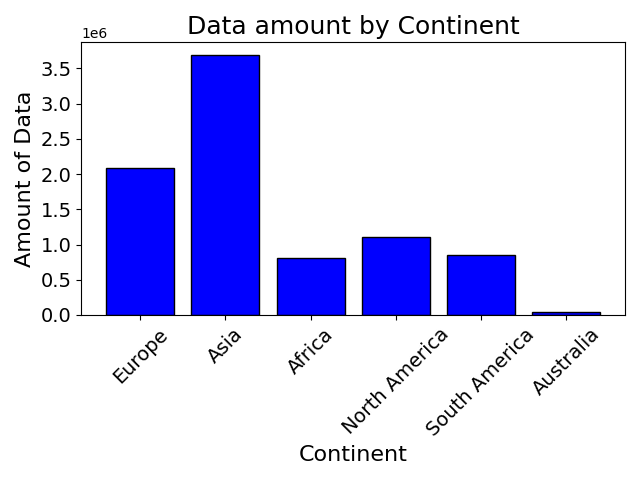
\includegraphics[width=.8\linewidth]{./histograms/Continents}
      \caption{Histogram 1}
      \label{fig:sub1}
  \end{subfigure}%
  \begin{subfigure}{.45\textwidth}
      \centering
      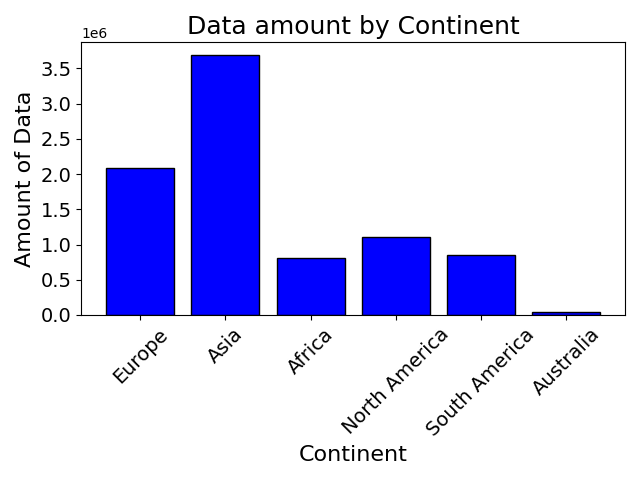
\includegraphics[width=.8\linewidth]{./histograms/Continents}
      \caption{Histogram 2}
      \label{fig:sub2}
  \end{subfigure}\\
  \begin{subfigure}{.45\textwidth}
      \centering
      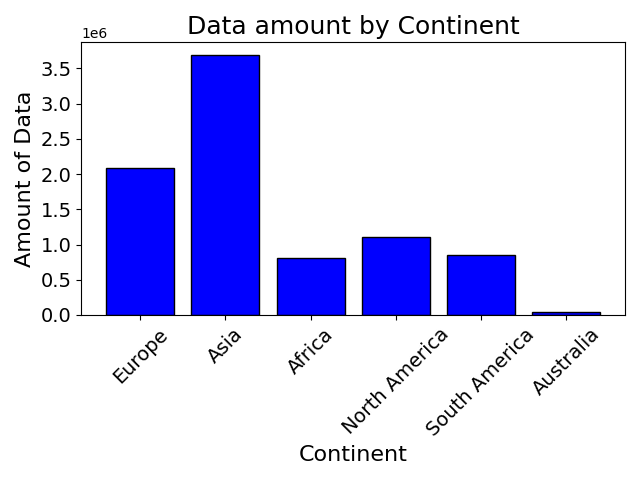
\includegraphics[width=.8\linewidth]{./histograms/Continents}
      \caption{Histogram 3}
      \label{fig:sub3}
  \end{subfigure}%
  \begin{subfigure}{.45\textwidth}
      \centering
      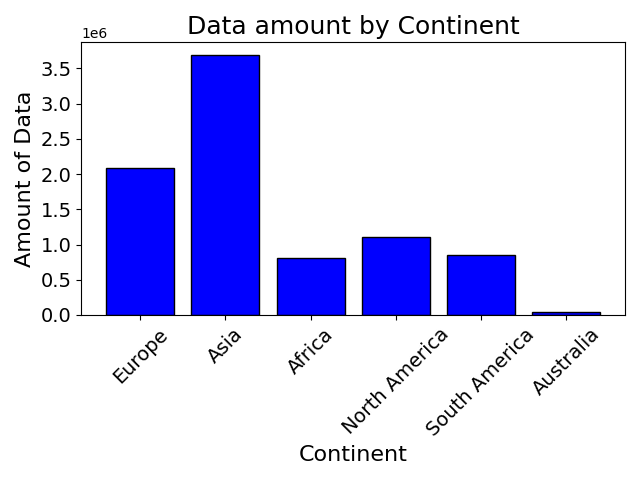
\includegraphics[width=.8\linewidth]{./histograms/Continents}
      \caption{Histogram 4}
      \label{fig:sub4}
  \end{subfigure}
  \caption{Four histograms}
  \label{fig:test}
  \Description{Histograms caputuring the distribution of the data.}
\end{figure}

Die Implementierung verschiedener Visualisierungen spielt eine entscheidende Rolle bei der Analyse von Daten und Vorhersagen. Hierbei wurden Histogramme für den Längen- und Breitengrad, die Verteilung von Datenlücken, Temperaturverteilungen und Unsicherheiten erstellt. Zusätzlich wurde ein Kartenplot der Datenpunkte generiert. Diese Visualisierungen bieten Einblicke in die geografische Verteilung der Daten und ermöglichen eine detaillierte Analyse von Städten mit identischen Werten.
\section{Data-Loader Pipeline und Visualisierungen}
Die Data-Loader Pipeline wurde implementiert, um Mini-Batches von Sequenzen von Datenpunkten gemäß den Anforderungen der Architekturen bereitzustellen. Dieser Prozess wurde optimiert, um die Effizienz des Trainings zu steigern. Zur Analyse wurden Visualisierungen wie Histogramme für geografische Merkmale, Datenverteilungen und Kartenplots verwendet. T-SNE-Plots ermöglichen eine multidimensionale Darstellung der Datenpunkte für eine bessere Analyse.
\section{Architekturvergleich und Normalisierungen}
Die Leistung der Architekturen wurde sowohl qualitativ als auch quantitativ bewertet. Aktivierungsfunktionen wie Selu und Relu wurden für MLP analysiert. Bei 1D Conv Net wurde die Auswirkung von Global Average Pooling und Flatten vor den Dense Layern untersucht. LSTM und Transformer wurden auf ihre spezifischen Eigenschaften und Fehlerquellen analysiert. Der Vergleich erfolgte durch Bewertung der qualitativen Anpassung und quantitativen Metriken wie dem Mean Absolute Error (MAE).
\section{Normalisierung und Variation der Input-Sequenzen}
Die Daten wurden vor dem Training normalisiert, und die Auswirkungen auf die Vorhersagegenauigkeit wurden verglichen. Zusätzlich wurde die Performance der Modelle für variable Input-Sequenzen von 8, 16, 32 und 64 untersucht. Dies ermöglichte eine tiefgreifende Analyse, wie die Länge der Input-Sequenzen die Modellleistung beeinflusst.


Insgesamt bietet diese Studie eine umfassende Analyse der Climate Change-Daten unter Verwendung verschiedener Netzwerkarchitekturen. Die gewonnenen Erkenntnisse ermöglichen nicht nur eine bessere Anpassung der Modelle an die Daten, sondern auch Optimierungsmöglichkeiten für zukünftige Forschungen im Bereich des Klimawandels.

\section{Citations and Bibliographies}

The use of \BibTeX\ for the preparation and formatting of one's
references is strongly recommended. Authors' names should be complete
--- use full first names (``Donald E. Knuth'') not initials
(``D. E. Knuth'') --- and the salient identifying features of a
reference should be included: title, year, volume, number, pages,
article DOI, etc.

The bibliography is included in your source document with these two
commands, placed just before the \verb|\end{document}| command:
\begin{verbatim}
  \bibliographystyle{ACM-Reference-Format}
  \bibliography{bibfile}
\end{verbatim}
where ``\verb|bibfile|'' is the name, without the ``\verb|.bib|''
suffix, of the \BibTeX\ file.

Citations and references are numbered by default. A small number of
ACM publications have citations and references formatted in the
``author year'' style; for these exceptions, please include this
command in the {\bfseries preamble} (before the command
``\verb|\begin{document}|'') of your \LaTeX\ source:
\begin{verbatim}
  \citestyle{acmauthoryear}
\end{verbatim}

  Some examples.  A paginated journal article \cite{Abril07}, an
  enumerated journal article \cite{Cohen07}, a reference to an entire
  issue \cite{JCohen96}, a monograph (whole book) \cite{Kosiur01}, a
  monograph/whole book in a series (see 2a in spec. document)
  \cite{Harel79}, a divisible-book such as an anthology or compilation
  \cite{Editor00} followed by the same example, however we only output
  the series if the volume number is given \cite{Editor00a} (so
  Editor00a's series should NOT be present since it has no vol. no.),
  a chapter in a divisible book \cite{Spector90}, a chapter in a
  divisible book in a series \cite{Douglass98}, a multi-volume work as
  book \cite{Knuth97}, a couple of articles in a proceedings (of a
  conference, symposium, workshop for example) (paginated proceedings
  article) \cite{Andler79, Hagerup1993}, a proceedings article with
  all possible elements \cite{Smith10}, an example of an enumerated
  proceedings article \cite{VanGundy07}, an informally published work
  \cite{Harel78}, a couple of preprints \cite{Bornmann2019,
    AnzarootPBM14}, a doctoral dissertation \cite{Clarkson85}, a
  master's thesis: \cite{anisi03}, an online document / world wide web
  resource \cite{Thornburg01, Ablamowicz07, Poker06}, a video game
  (Case 1) \cite{Obama08} and (Case 2) \cite{Novak03} and \cite{Lee05}
  and (Case 3) a patent \cite{JoeScientist001}, work accepted for
  publication \cite{rous08}, 'YYYYb'-test for prolific author
  \cite{SaeediMEJ10} and \cite{SaeediJETC10}. Other cites might
  contain 'duplicate' DOI and URLs (some SIAM articles)
  \cite{Kirschmer:2010:AEI:1958016.1958018}. Boris / Barbara Beeton:
  multi-volume works as books \cite{MR781536} and \cite{MR781537}. A
  couple of citations with DOIs:
  \cite{2004:ITE:1009386.1010128,Kirschmer:2010:AEI:1958016.1958018}. Online
  citations: \cite{TUGInstmem, Thornburg01, CTANacmart}. Artifacts:
  \cite{R} and \cite{UMassCitations}.

\section{Acknowledgments}

Identification of funding sources and other support, and thanks to
individuals and groups that assisted in the research and the
preparation of the work should be included in an acknowledgment
section, which is placed just before the reference section in your
document.

This section has a special environment:
\begin{verbatim}
  \begin{acks}
  ...
  \end{acks}
\end{verbatim}
so that the information contained therein can be more easily collected
during the article metadata extraction phase, and to ensure
consistency in the spelling of the section heading.

Authors should not prepare this section as a numbered or unnumbered {\verb|\section|}; please use the ``{\verb|acks|}'' environment.

\section{Appendices}

If your work needs an appendix, add it before the
``\verb|\end{document}|'' command at the conclusion of your source
document.

Start the appendix with the ``\verb|appendix|'' command:
\begin{verbatim}
  \appendix
\end{verbatim}
and note that in the appendix, sections are lettered, not
numbered. This document has two appendices, demonstrating the section
and subsection identification method.

\section{Multi-language papers}

Papers may be written in languages other than English or include
titles, subtitles, keywords and abstracts in different languages (as a
rule, a paper in a language other than English should include an
English title and an English abstract).  Use \verb|language=...| for
every language used in the paper.  The last language indicated is the
main language of the paper.  For example, a French paper with
additional titles and abstracts in English and German may start with
the following command
\begin{verbatim}
\documentclass[sigconf, language=english, language=german,
               language=french]{acmart}
\end{verbatim}

The title, subtitle, keywords and abstract will be typeset in the main
language of the paper.  The commands \verb|\translatedXXX|, \verb|XXX|
begin title, subtitle and keywords, can be used to set these elements
in the other languages.  The environment \verb|translatedabstract| is
used to set the translation of the abstract.  These commands and
environment have a mandatory first argument: the language of the
second argument.  See \verb|sample-sigconf-i13n.tex| file for examples
of their usage.

\section{SIGCHI Extended Abstracts}

The ``\verb|sigchi-a|'' template style (available only in \LaTeX\ and
not in Word) produces a landscape-orientation formatted article, with
a wide left margin. Three environments are available for use with the
``\verb|sigchi-a|'' template style, and produce formatted output in
the margin:
\begin{itemize}
\item {\verb|sidebar|}:  Place formatted text in the margin.
\item {\verb|marginfigure|}: Place a figure in the margin.
\item {\verb|margintable|}: Place a table in the margin.
\end{itemize}

%%
%% The acknowledgments section is defined using the "acks" environment
%% (and NOT an unnumbered section). This ensures the proper
%% identification of the section in the article metadata, and the
%% consistent spelling of the heading.
\begin{acks}
To Robert, for the bagels and explaining CMYK and color spaces.
\end{acks}

%%
%% The next two lines define the bibliography style to be used, and
%% the bibliography file.
\bibliographystyle{ACM-Reference-Format}
\bibliography{sample-base}

%%
%% If your work has an appendix, this is the place to put it.
\appendix

\section{Research Methods}

\subsection{Part One}

Lorem ipsum dolor sit amet, consectetur adipiscing elit. Morbi
malesuada, quam in pulvinar varius, metus nunc fermentum urna, id
sollicitudin purus odio sit amet enim. Aliquam ullamcorper eu ipsum
vel mollis. Curabitur quis dictum nisl. Phasellus vel semper risus, et
lacinia dolor. Integer ultricies commodo sem nec semper.

\subsection{Part Two}

Etiam commodo feugiat nisl pulvinar pellentesque. Etiam auctor sodales
ligula, non varius nibh pulvinar semper. Suspendisse nec lectus non
ipsum convallis congue hendrerit vitae sapien. Donec at laoreet
eros. Vivamus non purus placerat, scelerisque diam eu, cursus
ante. Etiam aliquam tortor auctor efficitur mattis.

\section{Online Resources}

Nam id fermentum dui. Suspendisse sagittis tortor a nulla mollis, in
pulvinar ex pretium. Sed interdum orci quis metus euismod, et sagittis
enim maximus. Vestibulum gravida massa ut felis suscipit
congue. Quisque mattis elit a risus ultrices commodo venenatis eget
dui. Etiam sagittis eleifend elementum.

Nam interdum magna at lectus dignissim, ac dignissim lorem
rhoncus. Maecenas eu arcu ac neque placerat aliquam. Nunc pulvinar
massa et mattis lacinia.

\end{document}
\endinput
%%
%% End of file `sample-authordraft.tex'.